\chapter{Results}

show comparision between all shader variants: pq, adaptive, all, nvidiaGem.
mention system specs and how long it took in order to precompute
mention GEM results.
show nminmax renderings

\begin{figure}[H]
  \centering
  \subfigure[A]{
    \includegraphics[scale=0.1118]{ElapheGuttata/1.png}
    \label{fig:realImageElapheGuttata1}
  }
~
  \subfigure[B]{
    \includegraphics[scale=0.189]{ElapheGuttata/4.png}
    \label{fig:realImageElapheGuttata2}
  }
  \label{realImageElapheGuttata}
  \caption{Species Elaphe Guttata}
\end{figure}

\begin{figure}[H]
  \centering
  \subfigure[A]{
    \includegraphics[scale=0.369]{XenopeltisUnicolor/2.png}
    \label{fig:realImageXeno1}
  }
~
  \subfigure[B]{
    \includegraphics[scale=0.40]{XenopeltisUnicolor/3.png}
    \label{fig:realImageXeno2}
  }
  \label{realImageXenopeltis}
  \caption{Species Xenopeltis Unicolor}
\end{figure}

Mention basic set up


brdf map for blazed grating shows typical high relative brightness for the first order of diffraction.

elaphe skin, finger-like nanostructure quite regularly placed, thus exhibits diffraction accros these periodic arrangements, i.e. there is a long horizontal axis for brdf map. furthermore fingers overlap across layers thus do not exhibit any definite periodicity along finger directions. hence do not see strong diffraction color along other directions in brdf map.

for xeno, layers of nano-fingers do not overlap and they manoeuvre significantly along their lenght but with some local consistency. thus see diffraction along many different directions in brdf map. similar argument for diffraction across locally periodic finger patches with slightly different orientations.


the elapse does not look that regular under the electron scanning microscope. This is why it is much less iridescent than the other specie.

In addition, the micro-geometry is highly similar among snake species, it is the geometry of the nanostructures that are highly different among species and that cause the snake to be or not be iridescent. So, even Xenopeltis would not give you very different geometry than Elaphe.

Xeno has a brownish body with no pattern that makes the iridescence more spectacular than on Ellaphe


\section{BRDF maps}
Following passage explains the structure of the partial BRD maps that are presented in this report. Consider a sample the partial BRD maps shown below :

\begin{figure}[H]
  \centering
  \subfigure[BRDF map schema]{
    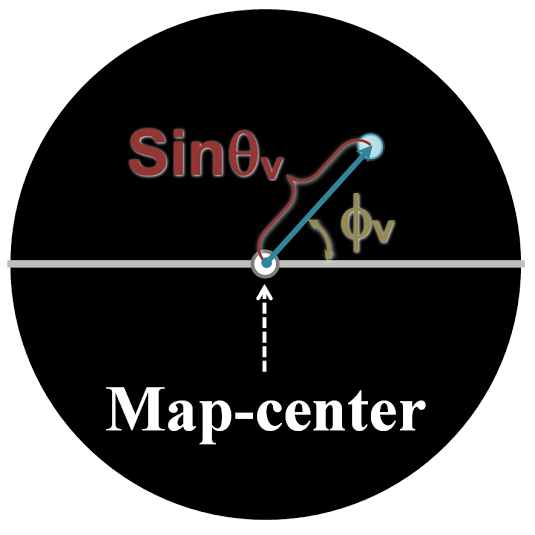
\includegraphics[scale=0.53]{results/brdfmapschema.png}
    \label{fig:brdfmapschema}
  }
~
  \subfigure[Light reflection geometrical setting]{
    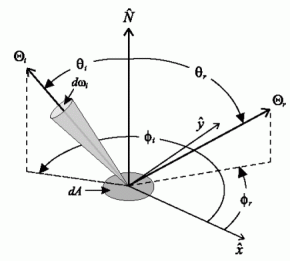
\includegraphics[scale=0.68]{results/Lightreflectiongeometry.png}
    \label{fig:lightreflectiongeometry}
  }
~

  \caption{BRDF maps for different patches: $\Theta=(\theta,\phi)$ is the direction of light propagation}
\label{fig:brdfmapexplanation}
\end{figure}

Distance from the center of the (circular) map = $sin(theta_r)$
Angle with the positive X-Axis in the map = $\phi_r$
$\theta_i$ and $\phi_i$ are constant for a given map, plot. For all the results presented in this report $\phi_i = \pi$


BRDF map shows shader output for all viewing directions and a fixed incident light direction. viewing direction represented in spherical coordinates $(\theta_v, \phi_v)$ is represented in map at point $(x,y) = (sin(\theta_v)cos(\phi_v), sin(\theta_v)sin(\phi_v))$ with origin at map center. fix light direction for normal incidence, i.e. $(\theta_i, \phi_i) = (0,0)$ unless specified otherwise. See figure $\ref{fig:brdfmapexplanation}$.

Mention brdf map basic idea figure + text


% brdf maps patches
\begin{figure}[H]
  \centering
  \subfigure[ALL lambda]{
    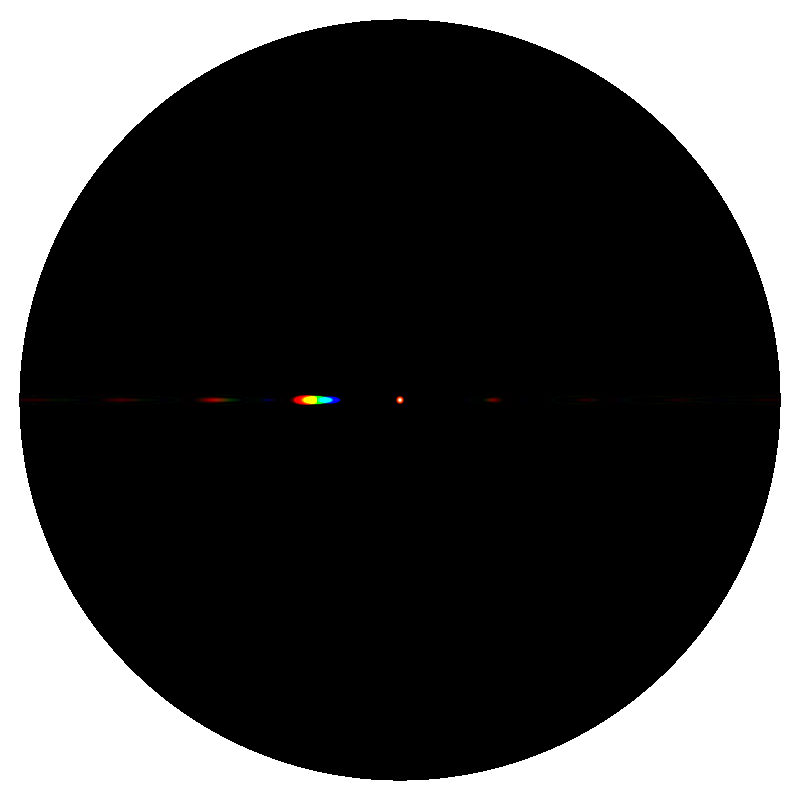
\includegraphics[scale=0.09]{results/diffPatches/fftBlazeHeight_0.25Microns_allL_weak_scale.png}
    \label{fig:brdfmapBlazeAllLambda}
  }
~
  \subfigure[Nmin Nmax]{
    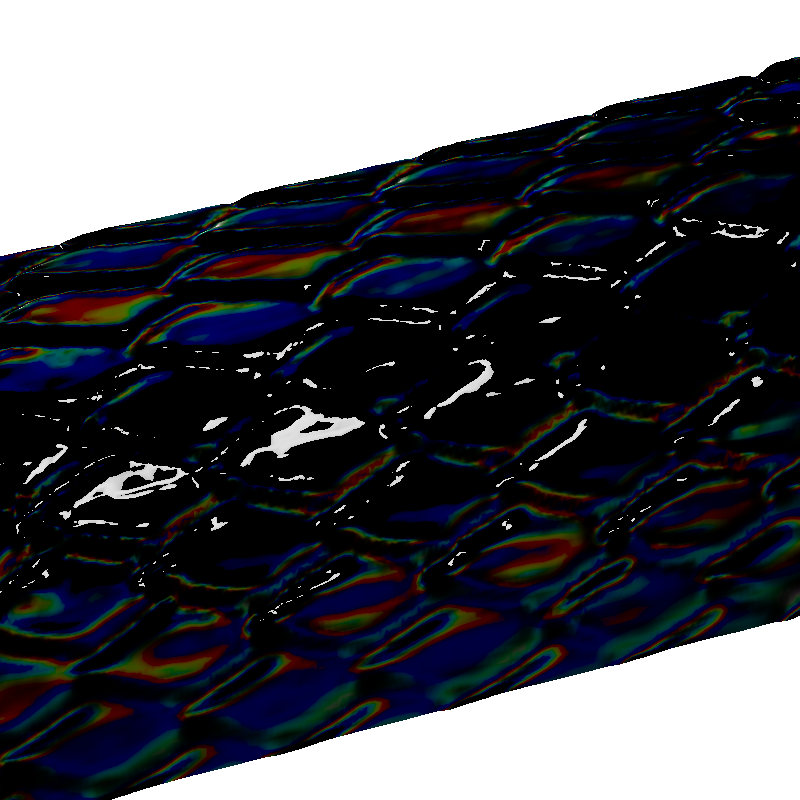
\includegraphics[scale=0.09]{results/methodComp/gem.png}
    \label{fig:brdfmapBlazeOnlyReq}
  }
~
  \subfigure[PQ]{
    \includegraphics[scale=0.09]{results/PQapproach_vs_sampleAll/blaze/pq.png}
    \label{fig:brdfmapBlazePQ}
  }
~
  \subfigure[Gem]{
    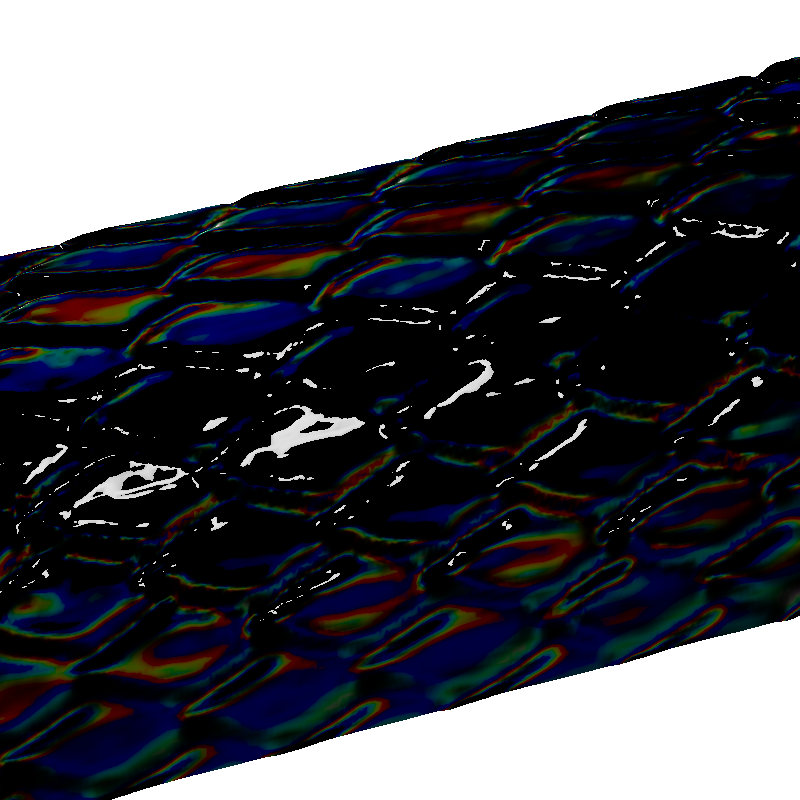
\includegraphics[scale=0.09]{results/methodComp/gem.png}
    \label{fig:brdfmapBlazeGem}
  }
  
  \label{brdfmapsDiffRenderingApproaches}
  \caption{BRDF maps for blaze grating comparing our different rendering apporaches}
\end{figure}

% add also a comp. for elaphe

brdf maps for different nanoscale surface gratings
% brdf maps patches
\begin{figure}[H]
  \centering
  \subfigure[Blaze grating]{
    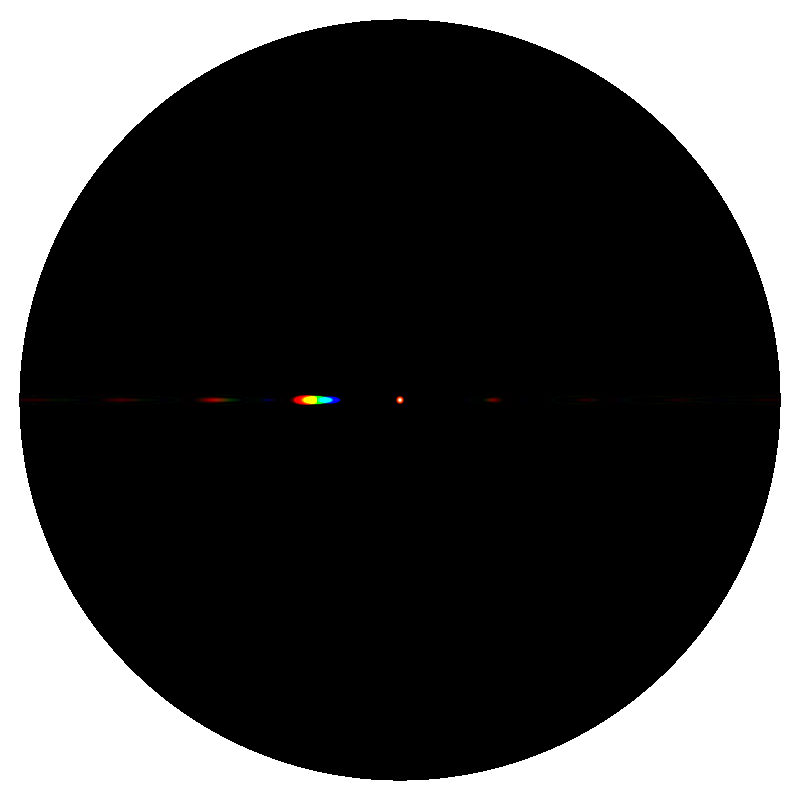
\includegraphics[scale=0.12]{results/diffPatches/fftBlazeHeight_0.25Microns_allL_weak_scale.png}
    \label{fig:brdfmapBlaze}
  }
~
  \subfigure[elaphe grating]{
    \includegraphics[scale=0.12]{results/diffPatches/elaph65.png}
    \label{fig:brdfmapElaphe}
  }
~
  \subfigure[xeno grating]{
    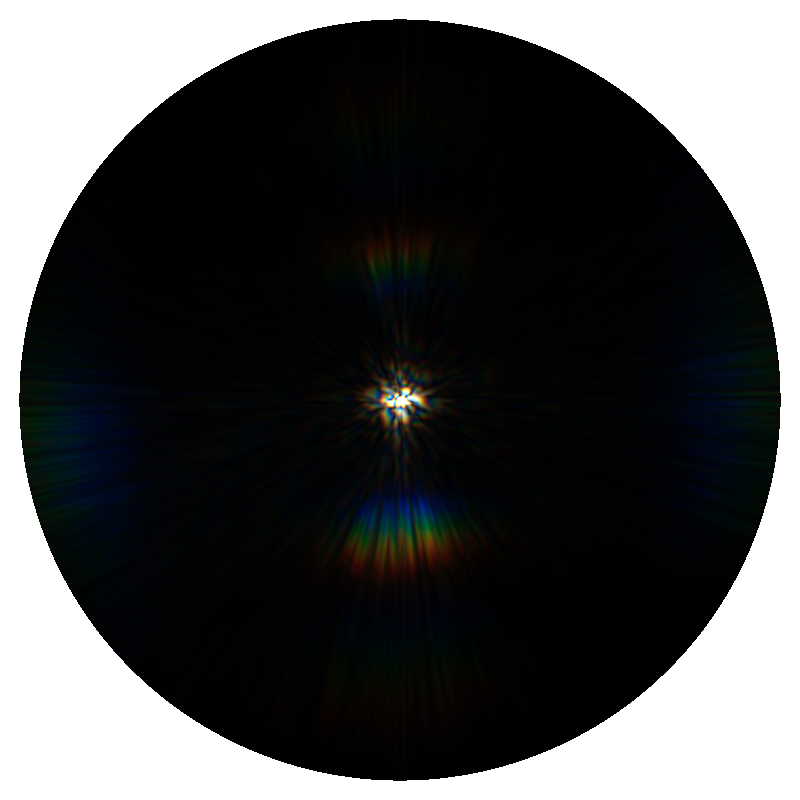
\includegraphics[scale=0.12]{results/diffPatches/xeno65.png}
    \label{fig:brdfmapXeno}
  }
  \label{brdfmapsDiffPatches}
  \caption{BRDF maps for different patches}
\end{figure}


for blaze grating different wavelength step sizes in fragment shader
wider steps fewer iterations, loss of qulatiy. for elaphe step bigger than 10nm there are visible artifacts. for blaze grating bigger step sizes possible. 
% blaze steps
\begin{figure}[H]
  \centering
  \subfigure[$\lambda_{step=1 nm}$]{
    \includegraphics[scale=0.12]{results/different_lambda_steps/blaze/dl=1.png}
    \label{fig:brdfmapsDiffLambdaStepsL1Blaze}
  }
~
  \subfigure[$\lambda_{step=5 nm}$]{
    \includegraphics[scale=0.12]{results/different_lambda_steps/blaze/dl=5.png}
    \label{fig:brdfmapsDiffLambdaStepsL5Blaze}
  }
~
  \subfigure[$\lambda_{step=10 nm}$]{
    \includegraphics[scale=0.12]{results/different_lambda_steps/blaze/dl=10.png}
    \label{fig:brdfmapsDiffLambdaStepsL10Blaze}
  }
  
  \subfigure[$\lambda_{step=25 nm}$]{
    \includegraphics[scale=0.12]{results/different_lambda_steps/blaze/dl=25.png}
    \label{fig:brdfmapsDiffLambdaStepsL25Blaze}
  }
~
  \subfigure[$\lambda_{step=50 nm}$]{
    \includegraphics[scale=0.12]{results/different_lambda_steps/blaze/dl=50.png}
    \label{fig:brdfmapsDiffLambdaStepsL50Blaze}
  }
~ 
  \subfigure[$\lambda_{step=100 nm}$]{
    \includegraphics[scale=0.12]{results/different_lambda_steps/blaze/dl=100.png}
    \label{fig:brdfmapsDiffLambdaStepsL100Blaze}
  }
  
  \label{brdfmapsDiffLambdaStepsBlaze}
  \caption{Blaze grating at $2.5 \mu m$: Different $\lambda$ step sizes}
\end{figure}

% elpahe steps
\begin{figure}[H]
  \centering
  \subfigure[$\lambda_{step=1 nm}$]{
    \includegraphics[scale=0.12]{results/different_lambda_steps/elaphe65/dl=1.png}
    \label{fig:brdfmapsDiffLambdaStepsL1Elaphe65}
  }
~
  \subfigure[$\lambda_{step=5 nm}$]{
    \includegraphics[scale=0.12]{results/different_lambda_steps/elaphe65/dl=5.png}
    \label{fig:brdfmapsDiffLambdaStepsL5Elaphe65}
  }
~
  \subfigure[$\lambda_{step=10 nm}$]{
    \includegraphics[scale=0.12]{results/different_lambda_steps/elaphe65/dl=10.png}
    \label{fig:brdfmapsDiffLambdaStepsL10Elaphe65}
  }
  
  \subfigure[$\lambda_{step=25 nm}$]{
    \includegraphics[scale=0.12]{results/different_lambda_steps/elaphe65/dl=25.png}
    \label{fig:brdfmapsDiffLambdaStepsL25Elaphe65}
  }
~
  \subfigure[$\lambda_{step=50 nm}$]{
    \includegraphics[scale=0.12]{results/different_lambda_steps/elaphe65/dl=50.png}
    \label{fig:brdfmapsDiffLambdaStepsL50Elaphe65}
  }
~ 
  \subfigure[$\lambda_{step=100 nm}$]{
    \includegraphics[scale=0.12]{results/different_lambda_steps/elaphe65/dl=100.png}
    \label{fig:brdfmapsDiffLambdaStepsL100Elaphe65}
  }
  
  \label{brdfmapsDiffLambdaStepsElaphe65}
  \caption{Elaphe grating at $65 \mu m$: Different $\lambda$ step sizes}
\end{figure}


compare pq qith full lambda sampling. see similarities but also differences 
%pq blaze
\begin{figure}[H]
  \centering
  \subfigure[Full Lambda Sampling: Blaze grating]{
    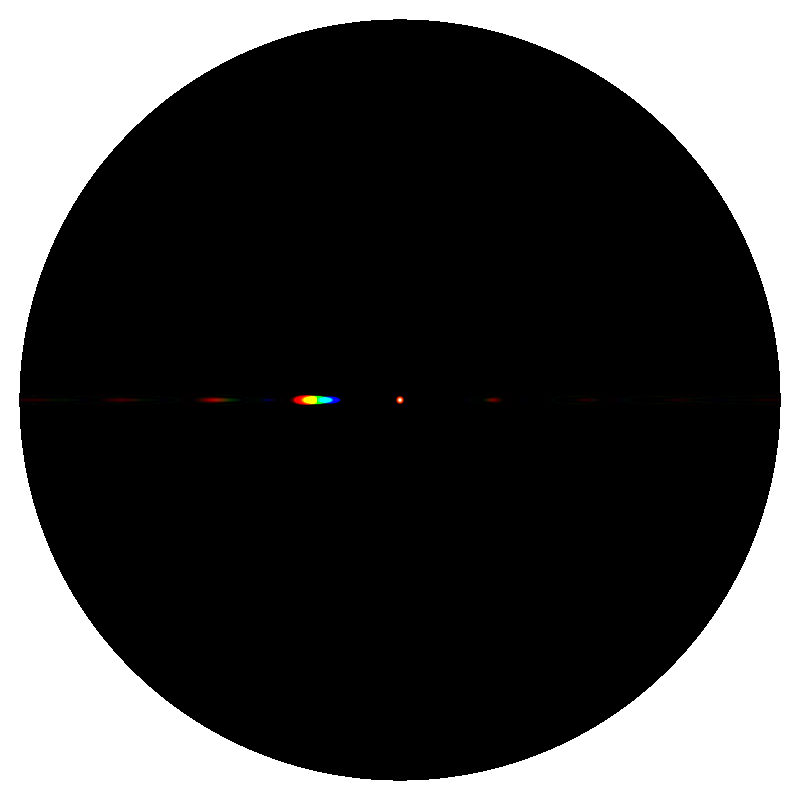
\includegraphics[scale=0.12]{results/PQapproach_vs_sampleAll/blaze/fftBlazeHeight_0.25Microns_allL_weak_scale_g=1.1.png}
    \label{fig:fullLambdaBlaze}
  }
~
  \subfigure[Full Lambda Sampling brightened: Blaze grating]{
    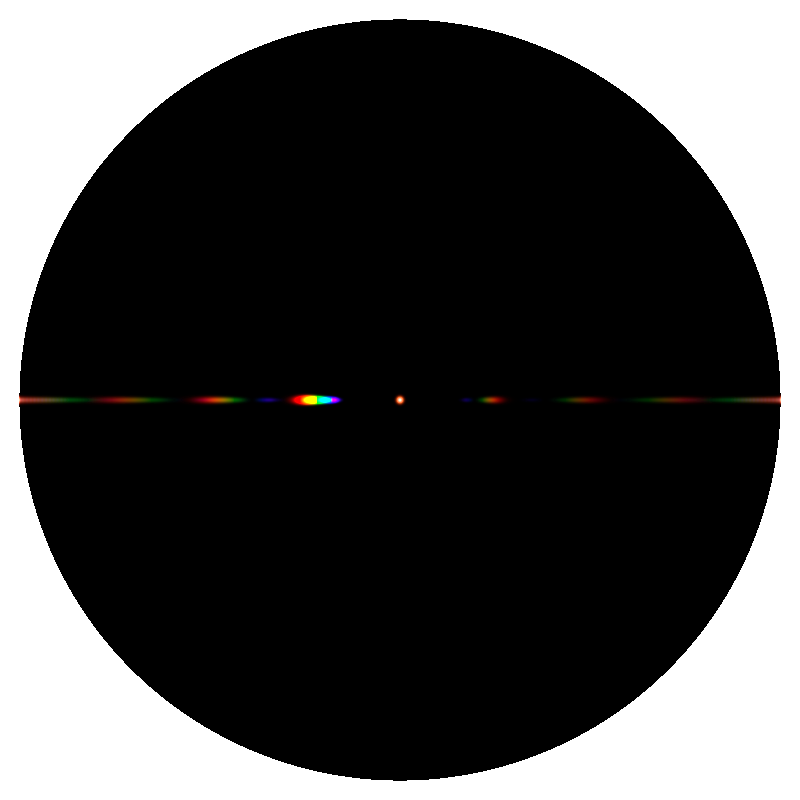
\includegraphics[scale=0.12]{results/PQapproach_vs_sampleAll/blaze/fftBlazeHeight_0.25Microns_allL_weak_scale_g=2.2_scale=100.png}
    \label{fig:fullLambdaBrightenedBlaze}
  }
~
  \subfigure[PQ Approach: Blaze grating]{
    \includegraphics[scale=0.12]{results/PQapproach_vs_sampleAll/blaze/pq.png}
    \label{fig:pqBlaze}
  }
  \label{pqBlaze}
  \caption{Blaze grating: PQ approach vs full lambda space sampling}
\end{figure}


%pq xeno
\begin{figure}[H]
  \centering
  \subfigure[Full Lambda Sampling: Xeno grating $\theta_i = 0 degree$]{
    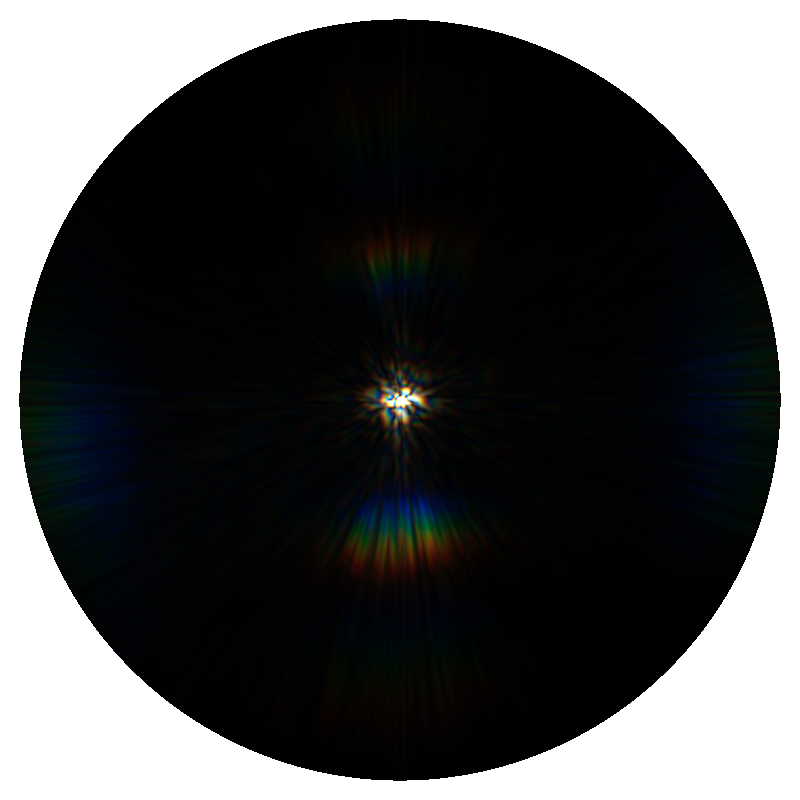
\includegraphics[scale=0.19]{results/PQapproach_vs_sampleAll/xeno/a_xeno_t_i=0.png}
    \label{fig:fullLambdaXenoti0}
  }
~
  \subfigure[PQ Approach: Xeno grating $\theta_i = 0 degree$]{
    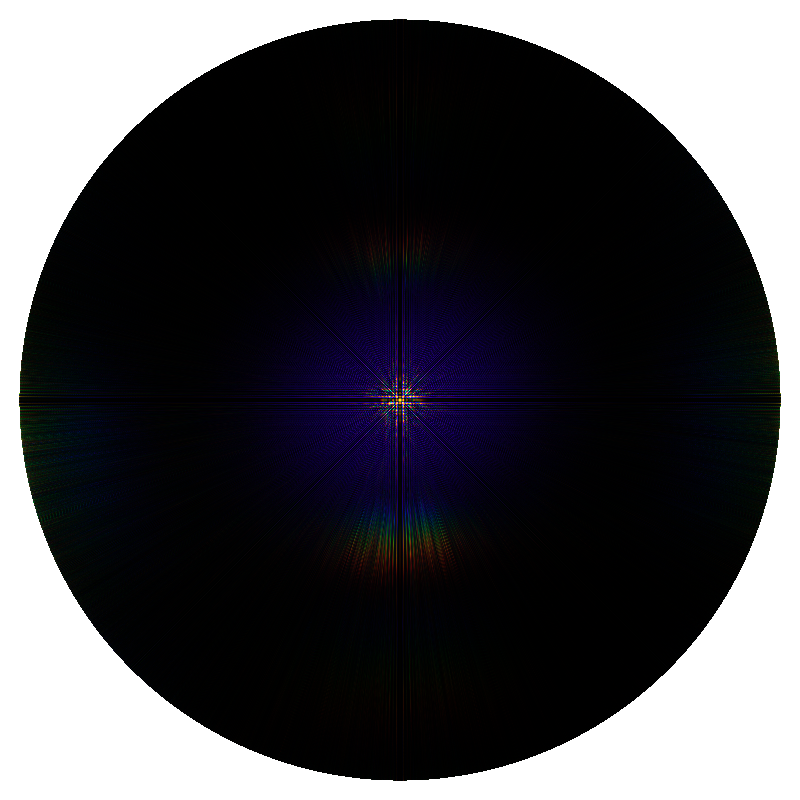
\includegraphics[scale=0.19]{results/PQapproach_vs_sampleAll/xeno/a_pq_t_i=0.png}
    \label{fig:pqXenoti0}
  }

  \subfigure[Full Lambda Sampling: Xeno grating $\theta_i = 10 degree$]{
    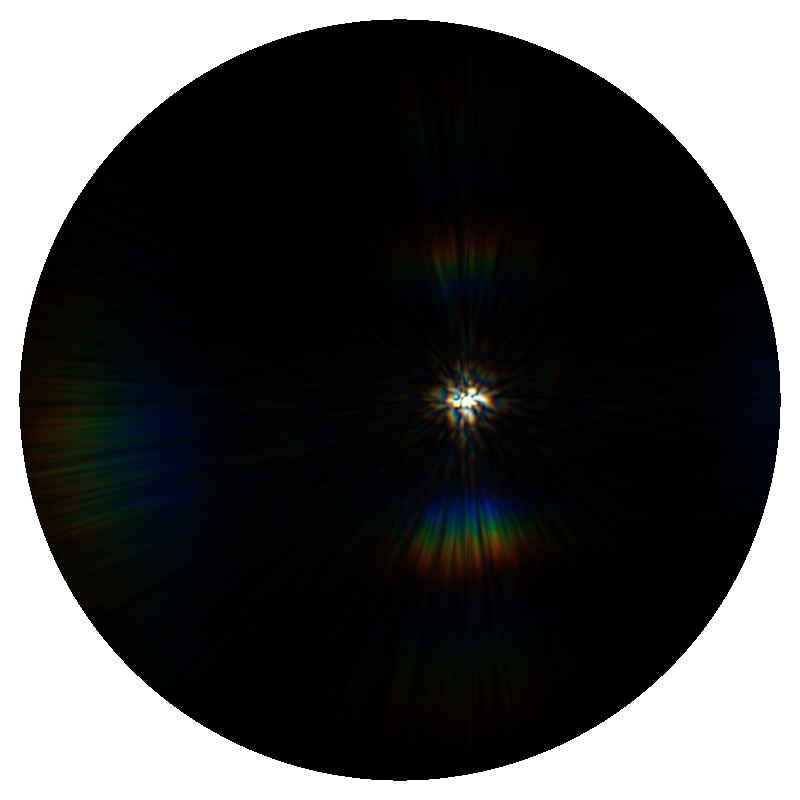
\includegraphics[scale=0.19]{results/PQapproach_vs_sampleAll/xeno/b_xeno_t_i=10.png}
    \label{fig:fullLambdaXenoti10}
  }
~
  \subfigure[PQ Approach: Xeno grating $\theta_i = 10 degree$]{
    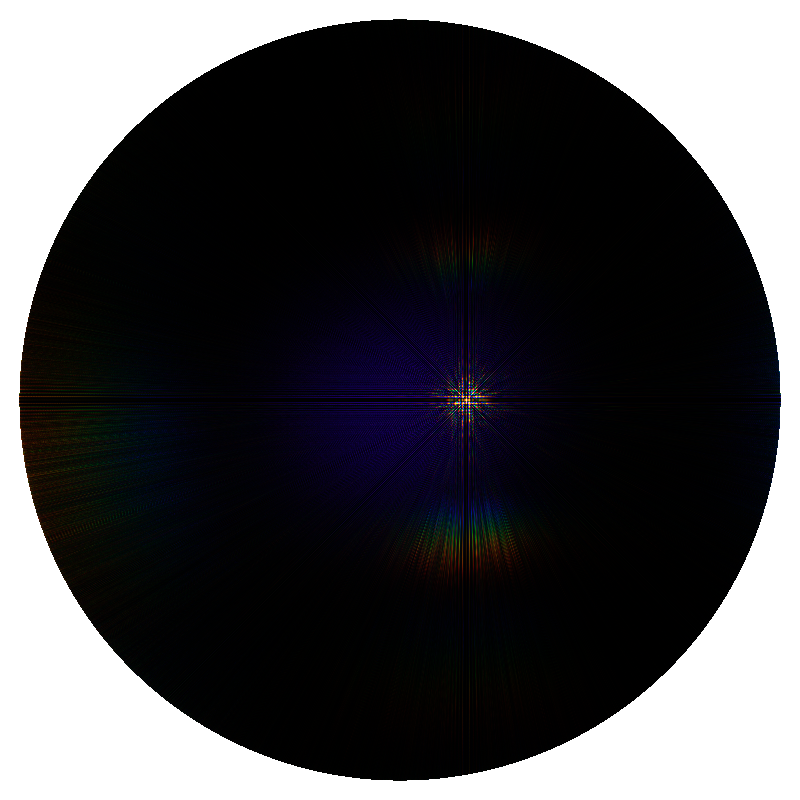
\includegraphics[scale=0.19]{results/PQapproach_vs_sampleAll/xeno/b_pq_t_i=10.png}
    \label{fig:pqXenoti10}
  }
  
  \subfigure[Full Lambda Sampling: Xeno grating $\theta_i = 20 degree$]{
    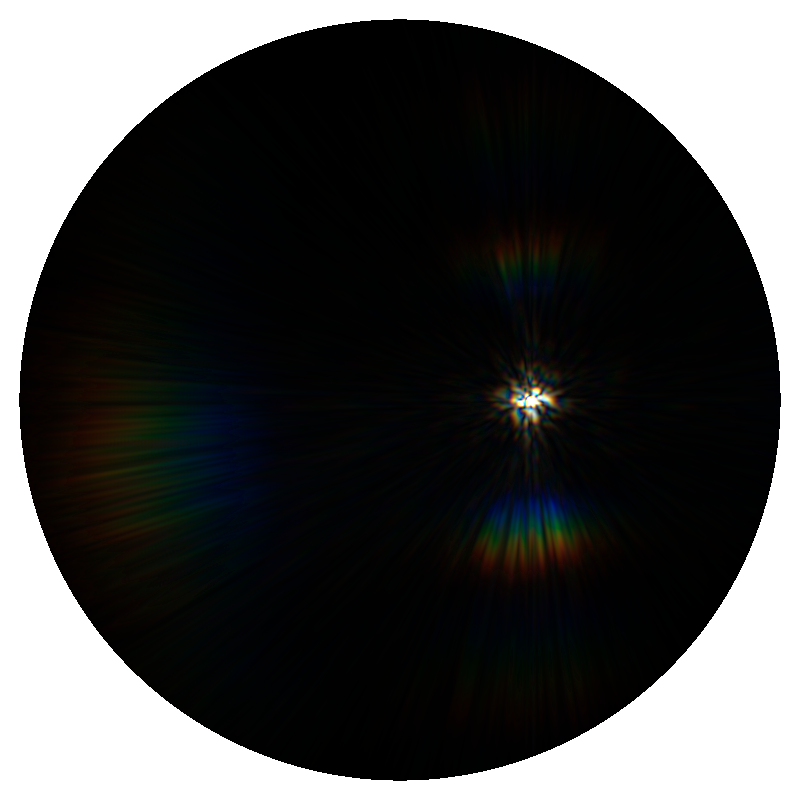
\includegraphics[scale=0.19]{results/PQapproach_vs_sampleAll/xeno/c_xeno_t_i=20.png}
    \label{fig:fullLambdaXenoti20}
  }
~
  \subfigure[PQ Approach: Xeno grating $\theta_i = 20 degree$]{
    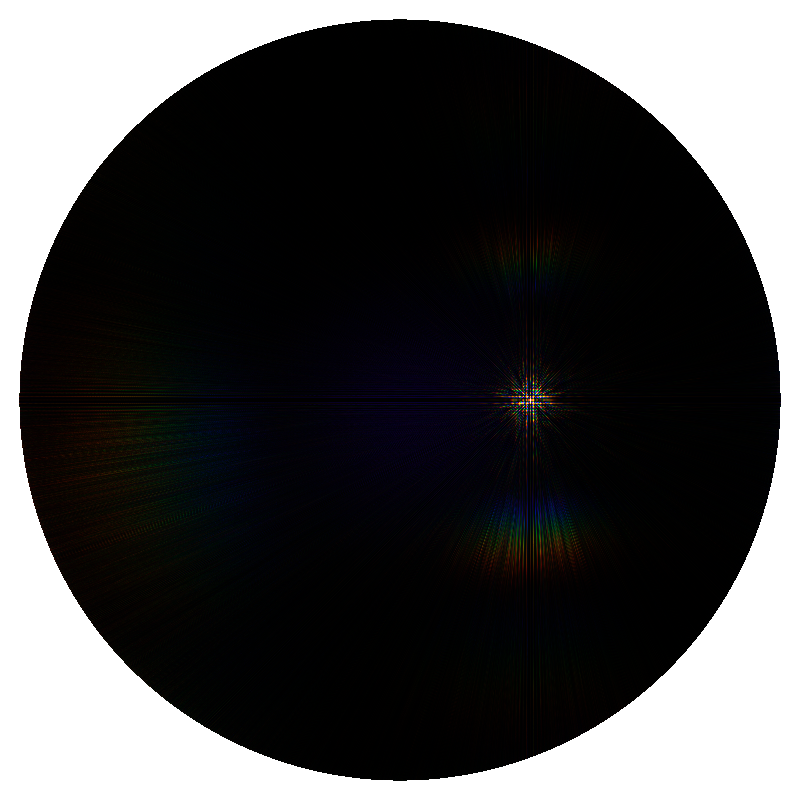
\includegraphics[scale=0.19]{results/PQapproach_vs_sampleAll/xeno/c_pq_t_i=20.png}
    \label{fig:pqXenoti20}
  }
  \label{pqXeno}
  \caption{Xeno grating: PQ approach vs full lambda space sampling}
\end{figure}

%pq elaphe
\begin{figure}[H]
  \centering
  \subfigure[Full Lambda Sampling: Elaphe grating]{
    \includegraphics[scale=0.2]{results/PQapproach_vs_sampleAll/elaphe/elaph65.png}
    \label{fig:fullLambdaElaphe}
  }
~
  \subfigure[PQ Approach: Elaphe grating]{
    \includegraphics[scale=0.2]{results/PQapproach_vs_sampleAll/elaphe/pq.png}
    \label{fig:pqElaphe}
  }

  \label{pqElaphe}
  \caption{Elaphe grating: PQ approach vs full lambda space sampling}
\end{figure}

blaze grating lower coherence length, fewer interacting grating periods, produce blurred diffraction bands for different lambda which overlap to produce poorly resolved colors.

%sigma var
\begin{figure}[H]
  \centering
  \subfigure[$\sigma_{s=3.25 \mu m}$]{
    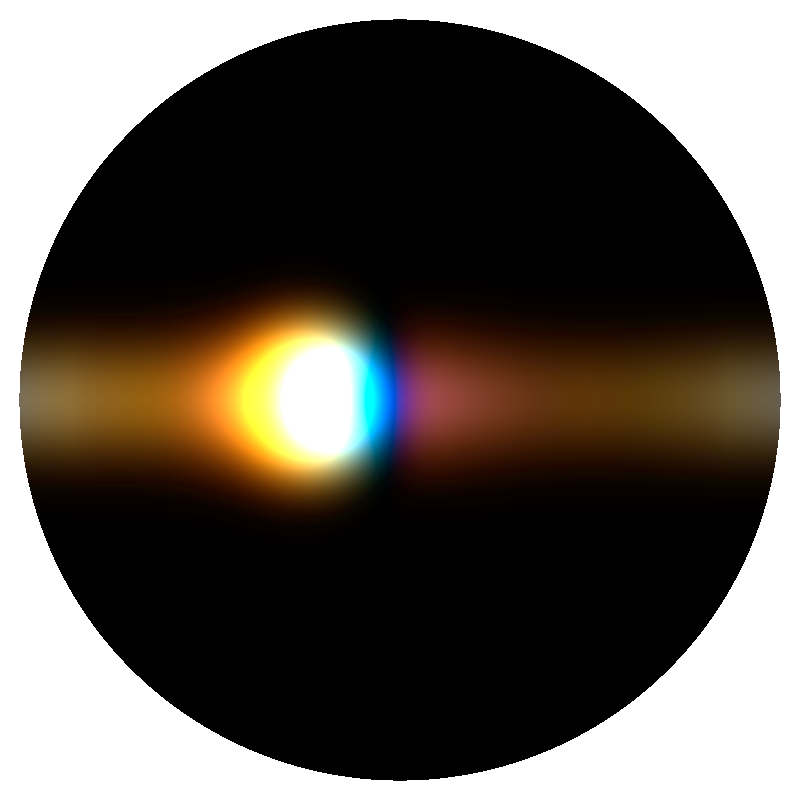
\includegraphics[scale=0.12]{results/sigma_sVariation/blaze/sigma_s=3.25.png}
    \label{fig:brdfmapsDiffSigmaStepsL1Blaze}
  }
~
  \subfigure[$\sigma_{s=6.5 \mu m}$]{
    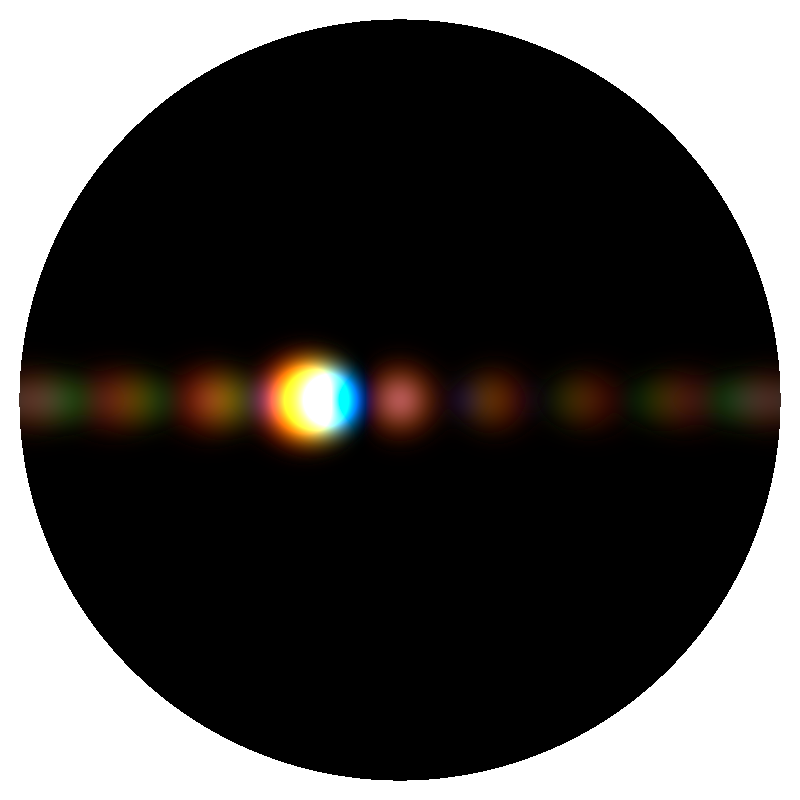
\includegraphics[scale=0.12]{results/sigma_sVariation/blaze/sigma_s=6.5.png}
    \label{fig:brdfmapsDiffSigmaStepsL5Blaze}
  }
~
  \subfigure[$\sigma_{s=15 \mu m}$]{
    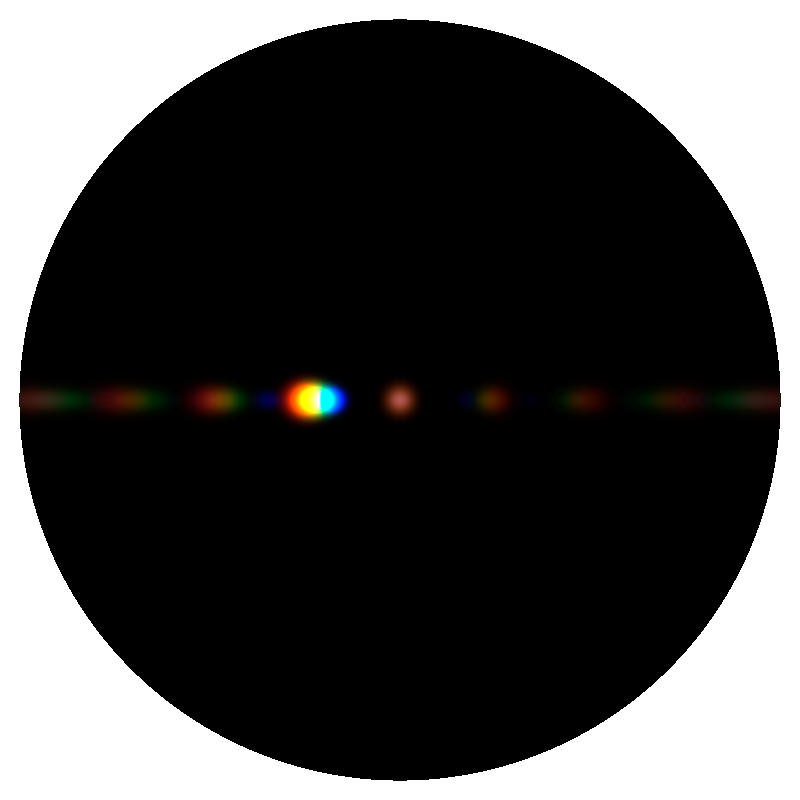
\includegraphics[scale=0.12]{results/sigma_sVariation/blaze/sigma_s=15.png}
    \label{fig:brdfmapsDiffSigmaStepsL10Blaze}
  }
  
  \subfigure[$\sigma_{s=30 \mu m}$]{
    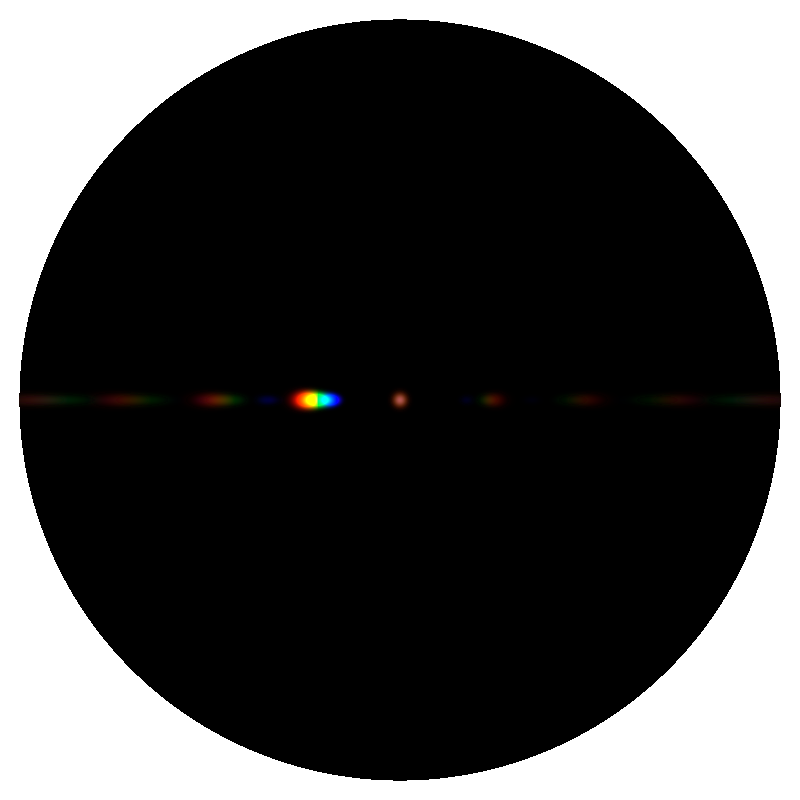
\includegraphics[scale=0.12]{results/sigma_sVariation/blaze/sigma_s=30.png}
    \label{fig:brdfmapsDiffSigmaStepsL25Blaze}
  }
~
  \subfigure[$\sigma_{s=45 \mu m}$]{
    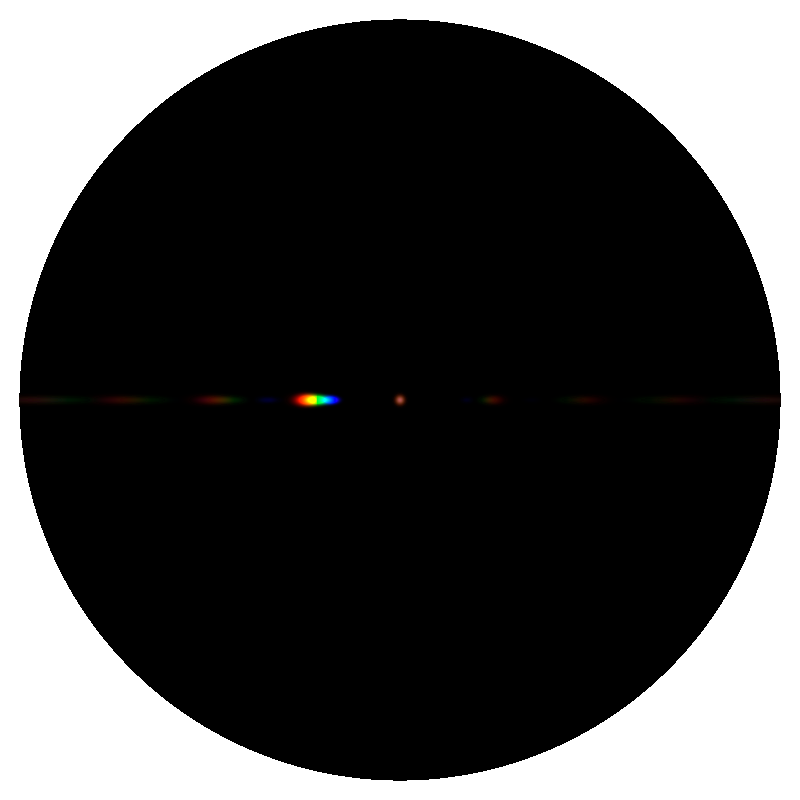
\includegraphics[scale=0.12]{results/sigma_sVariation/blaze/sigma_s=45.png}
    \label{fig:brdfmapsDiffSigmaStepsL50Blaze}
  }
~ 
  \subfigure[$\sigma_{s=65 \mu m}$]{
    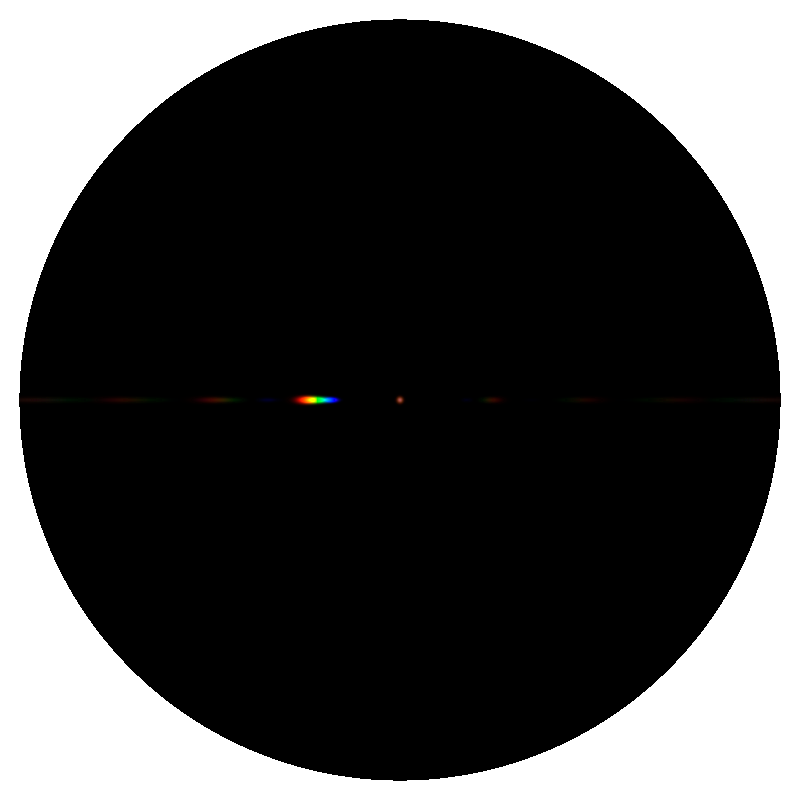
\includegraphics[scale=0.12]{results/sigma_sVariation/blaze/sigma_s=65.png}
    \label{fig:brdfmapsDiffSigmaStepsL100Blaze}
  }
  
  \label{brdfmapsDiffSigmaSizeBlaze}
  \caption{Blaze grating at $2.5 \mu m$: Different $\sigma_s$ sizes}
\end{figure}

visually convergence taylor series for higher values for N.

%taylor var elaphe
\begin{figure}[H]
  \centering
  \subfigure[$N=0$]{
    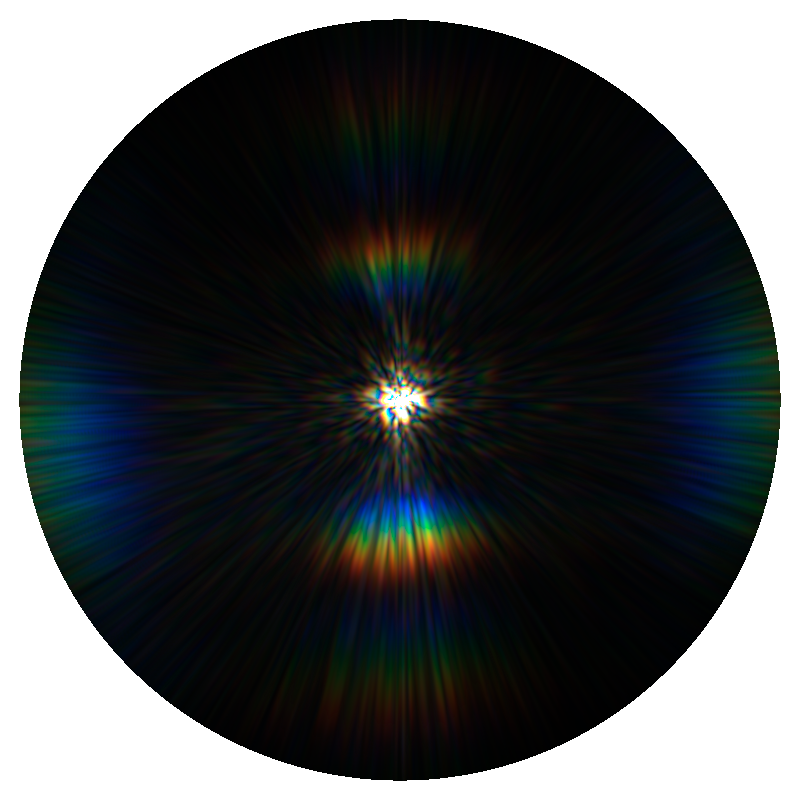
\includegraphics[scale=0.06]{results/taylorStepsVar/elaphe65/0.png}
    \label{fig:brdfmapsTaylorN0Elaphe65}
  }
~
  \subfigure[$N=1$]{
    \includegraphics[scale=0.06]{results/taylorStepsVar/elaphe65/1.png}
    \label{fig:brdfmapsTaylorN1Elaphe65}
  }
~
  \subfigure[$N=2$]{
    \includegraphics[scale=0.06]{results/taylorStepsVar/elaphe65/2.png}
    \label{fig:brdfmapsTaylorN2Elaphe65}
  }
~  
  \subfigure[$N=3$]{
    \includegraphics[scale=0.06]{results/taylorStepsVar/elaphe65/3.png}
    \label{fig:brdfmapsTaylorN3Elaphe65}
  }
~
  \subfigure[$N=4$]{
    \includegraphics[scale=0.06]{results/taylorStepsVar/elaphe65/4.png}
    \label{fig:brdfmapsTaylorN4Elaphe65}
  }

  \subfigure[$N=5$]{
    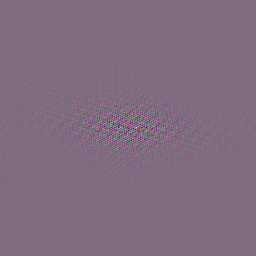
\includegraphics[scale=0.06]{results/taylorStepsVar/elaphe65/5.png}
    \label{fig:brdfmapsTaylorN5Elaphe65}
  }
~  
  \subfigure[$N=6$]{
    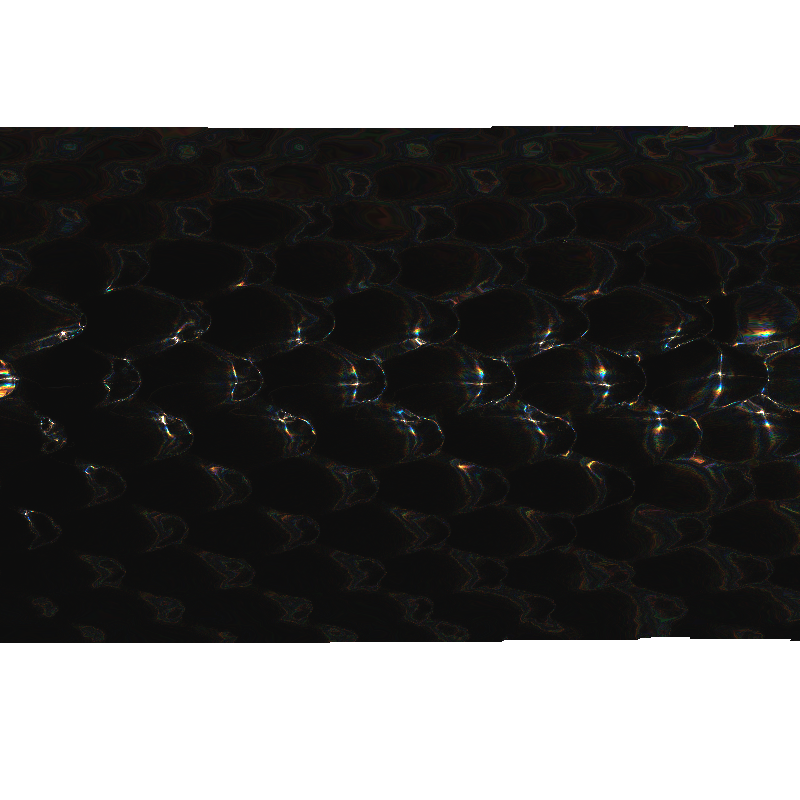
\includegraphics[scale=0.06]{results/taylorStepsVar/elaphe65/6.png}
    \label{fig:brdfmapsTaylorN6Elaphe65}
  }
~  
  \subfigure[$N=7$]{
    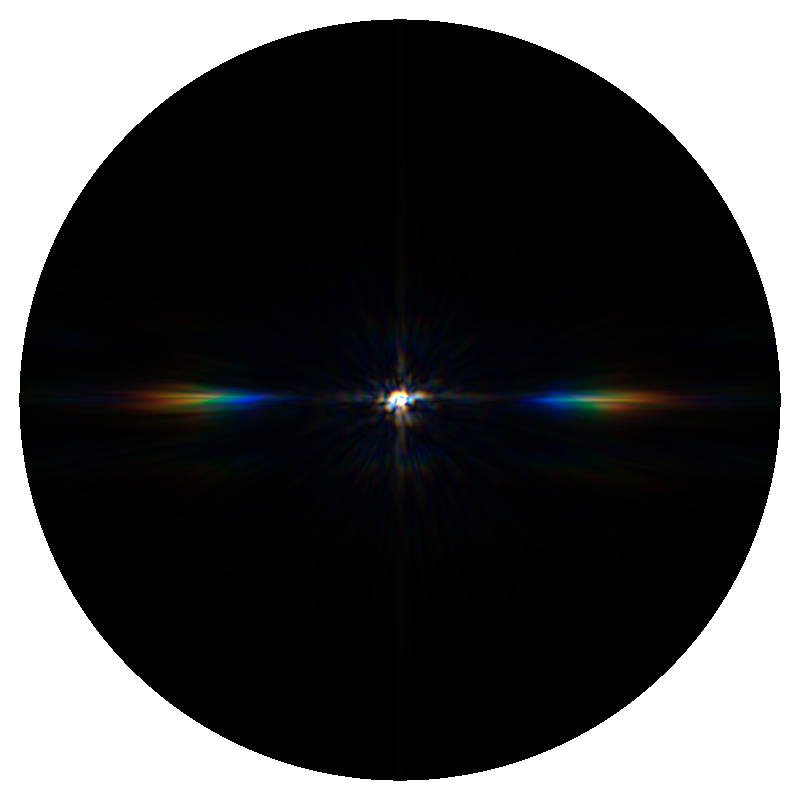
\includegraphics[scale=0.06]{results/taylorStepsVar/elaphe65/7.png}
    \label{fig:brdfmapsTaylorN7Elaphe65}
  }
~  
  \subfigure[$N=8$]{
    \includegraphics[scale=0.06]{results/taylorStepsVar/elaphe65/8.png}
    \label{fig:brdfmapsTaylorN8Elaphe65}
  }
~ 
  \subfigure[$N=9$]{
    \includegraphics[scale=0.06]{results/taylorStepsVar/elaphe65/9.png}
    \label{fig:brdfmapsTaylorN9Elaphe65}
  }
  
  \label{brdfmapsTaylorIterationsElaphe65}
  \caption{Elaphe grating at $65 \mu m$: $N$ Taylor Iterations}
\end{figure}


%taylor var blaze
\begin{figure}[H]
  \centering
  \subfigure[$N=0$]{
    \includegraphics[scale=0.06]{results/taylorStepsVar/blaze/0.png}
    \label{fig:brdfmapsTaylorN0Blaze}
  }
~
  \subfigure[$N=1$]{
    \includegraphics[scale=0.06]{results/taylorStepsVar/blaze/1.png}
    \label{fig:brdfmapsTaylorN1Blaze}
  }
~
  \subfigure[$N=2$]{
    \includegraphics[scale=0.06]{results/taylorStepsVar/blaze/2.png}
    \label{fig:brdfmapsTaylorN2Blaze}
  }
~  
  \subfigure[$N=3$]{
    \includegraphics[scale=0.06]{results/taylorStepsVar/blaze/3.png}
    \label{fig:brdfmapsTaylorN3Blaze}
  }
~
  \subfigure[$N=4$]{
    \includegraphics[scale=0.06]{results/taylorStepsVar/blaze/4.png}
    \label{fig:brdfmapsTaylorN4Blaze}
  }

  \subfigure[$N=5$]{
    \includegraphics[scale=0.06]{results/taylorStepsVar/blaze/5.png}
    \label{fig:brdfmapsTaylorN5Blaze}
  }
~  
  \subfigure[$N=6$]{
    \includegraphics[scale=0.06]{results/taylorStepsVar/blaze/6.png}
    \label{fig:brdfmapsTaylorN6Blaze}
  }
~  
  \subfigure[$N=7$]{
    \includegraphics[scale=0.06]{results/taylorStepsVar/blaze/7.png}
    \label{fig:brdfmapsTaylorN7Blaze}
  }
~  
  \subfigure[$N=8$]{
    \includegraphics[scale=0.06]{results/taylorStepsVar/blaze/8.png}
    \label{fig:brdfmapsTaylorN8Blaze}
  }
~ 
  \subfigure[$N=9$]{
    \includegraphics[scale=0.06]{results/taylorStepsVar/blaze/9.png}
    \label{fig:brdfmapsTaylorN9Blaze}
  }
  
  \label{brdfmapsTaylorIterationsBlaze}
  \caption{Blaze grating at $2.5 \mu m$: $N$ Taylor Iterations}
\end{figure}

% brdf maps xeno angles
\begin{figure}[H]
  \centering
  \subfigure[Xeno grating $\theta_i=0$]{
    \includegraphics[scale=0.12]{results/different_theta_i_angles/xenopeltis/xeno_t_i=0.png}
    \label{fig:brdfmapXenoti0}
  }
~
  \subfigure[Xeno grating $\theta_i=10$]{
    \includegraphics[scale=0.12]{results/different_theta_i_angles/xenopeltis/xeno_t_i=10.png}
    \label{fig:brdfmapXenoti10}
  }
~
  \subfigure[Xeno grating $\theta_i=20$]{
    \includegraphics[scale=0.12]{results/different_theta_i_angles/xenopeltis/xeno_t_i=20.png}
    \label{fig:brdfmapXenoti20}
  }
  \label{brdfmapsXenoDiffThetaIAngles}
  \caption{BRDF maps for Xeno grating: different $\theta_i$ angles}
\end{figure}


\section{Snake surface geometries}
initially using fully lambda shader for those renderings, slow but accurate.

diffraction colors change dramatically with changes in light direction, surface normals and viewing direction, which s typical for diffraction colors observed in nature.

Mention resuolution of patches and their runtimes with used hardware - specify this hardware too.

\begin{figure}[H]
  \centering
  \subfigure[Blaze grating]{
    \includegraphics[scale=0.12]{results/snakerenderings/compars/blaze.png}
    \label{fig:renderingBlazeGrating}
  }
~
  \subfigure[Elaphe grating]{
    \includegraphics[scale=0.12]{results/snakerenderings/compars/elaphe65.png}
    \label{fig:renderingElapheGrating}
  }
~
  \subfigure[Xeno grating]{
    \includegraphics[scale=0.12]{results/snakerenderings/compars/xeno65.png}
    \label{fig:renderingXenoGrating}
  }
  \label{renderingDifferentSnankeGratings}
  \caption{Diffraction of different snake skin gratings rendered on a snake geometry}
\end{figure}


\begin{figure}[H]
  \centering
  \subfigure[$zoom = 0.1$]{
    \includegraphics[scale=0.2]{results/snakerenderings/zoomIn/elaphe65/0.1.png}
    \label{fig:renderingZoomElaphe01}
  }
~
  \subfigure[$zoom = 0.2$]{
    \includegraphics[scale=0.2]{results/snakerenderings/zoomIn/elaphe65/0.2.png}
    \label{fig:renderingZoomElaphe02}
  }
  
  \subfigure[$zoom = 0.5$]{
    \includegraphics[scale=0.2]{results/snakerenderings/zoomIn/elaphe65/0.5.png}
    \label{fig:renderingZoomElaphe05}
  }
~
  \subfigure[$zoom = 1.0$]{
    \includegraphics[scale=0.2]{results/snakerenderings/zoomIn/elaphe65/1.png}
    \label{fig:renderingZoomElaphe1}
  }
  
  \subfigure[$zoom = 1.5$]{
    \includegraphics[scale=0.2]{results/snakerenderings/zoomIn/elaphe65/1.5.png}
    \label{fig:renderingZoomElaphe15}
  }
~
  \subfigure[$zoom = 2.0$]{
    \includegraphics[scale=0.2]{results/snakerenderings/zoomIn/elaphe65/2.png}
    \label{fig:renderingZoomElaphe2}
  }
  \label{renderingDifferentZoomLevelsElaphe}
  \caption{Diffraction on Elaphe snake skin grating: Different camera zoom levels}
\end{figure}

% first 3 move along x, next 3 move along y
\begin{figure}[H]
  \centering
  \subfigure[$(-3.3130, 0.0, -0.9999)$]{
    \includegraphics[scale=0.12]{results/snakerenderings/rotateLight/elaphe65/moveX/2.png}
    \label{fig:renderingElapheRotX2}
  }
~
  \subfigure[$(-0.1989, 0.0, -0.9799)$]{
    \includegraphics[scale=0.12]{results/snakerenderings/rotateLight/elaphe65/moveX/4.png}
    \label{fig:renderingElapheRotX4}
  }
~
  \subfigure[$(-0.3897, 0.0, -0.9208)$]{
    \includegraphics[scale=0.12]{results/snakerenderings/rotateLight/elaphe65/moveX/6.png}
    \label{fig:renderingElapheRotX6}
  }
  
  \subfigure[$(0.0995, 0.0993, -0.9900)$]{
    \includegraphics[scale=0.12]{results/snakerenderings/rotateLight/elaphe65/moveY/2.png}
    \label{fig:renderingElapheRotY2}
  }
~
  \subfigure[$(0.0995, 0.2940, -0.9505)$]{
    \includegraphics[scale=0.12]{results/snakerenderings/rotateLight/elaphe65/moveY/4.png}
    \label{fig:renderingElapheRotY4}
  }
~
  \subfigure[$(0.0995, 0.4770, -0.8731)$]{
    \includegraphics[scale=0.12]{results/snakerenderings/rotateLight/elaphe65/moveY/6.png}
    \label{fig:renderingElapheRotY6}
  }
  
  \label{renderingElapheLightRotations6}
  \caption{Diffraction on Elaphe snake skin grating: Different light directions}
\end{figure}

\begin{figure}[H]
  \centering
  \subfigure[Diffraction Patten]{
    \includegraphics[scale=0.2]{results/snakerenderings/elaphe65/1.png}
    \label{fig:renderingElaphe65DP}
  }
~
  \subfigure[Diffraction + Texture]{
    \includegraphics[scale=0.2]{results/snakerenderings/elaphe65/2.png}
    \label{fig:renderingElaphe65DT}
  }

  \subfigure[Texture + Lightdir]{
    \includegraphics[scale=0.12]{results/snakerenderings/elaphe65/3.png}
    \label{fig:renderingElaphe65TL}
  }
~
  \subfigure[Nanostructure]{
    \includegraphics[scale=0.10]{results/snakerenderings/elaphe65/4.png}
    \label{fig:renderingElaphe65NS}
  }
~ 
  \subfigure[Fourier Transform]{
    \includegraphics[scale=0.52]{results/snakerenderings/elaphe65/5.png}
    \label{fig:renderingElaphe65FT}
  }
  
  
  \label{renderingElaphe65}
  \caption{Diffraction for Elaphe snake skin}
\end{figure}


\begin{figure}[H]
  \centering
  \subfigure[Diffraction Patten]{
    \includegraphics[scale=0.2]{results/snakerenderings/xeno65/1.png}
    \label{fig:renderingXeno65DP}
  }
~
  \subfigure[Diffraction + Texture]{
    \includegraphics[scale=0.2]{results/snakerenderings/xeno65/2.png}
    \label{fig:renderingXeno65DT}
  }

  \subfigure[Texture + Lightdir]{
    \includegraphics[scale=0.12]{results/snakerenderings/xeno65/3.png}
    \label{fig:renderingXeno65TL}
  }
~
  \subfigure[Nanostructure]{
    \includegraphics[scale=0.075]{results/snakerenderings/xeno65/4.png}
    \label{fig:renderingXeno65NS}
  }
~ 
  \subfigure[Fourier Transform]{
    \includegraphics[scale=0.52]{results/snakerenderings/xeno65/5.png}
    \label{fig:renderingXeno65FT}
  }
  
  
  \label{renderingXeno65}
  \caption{Diffraction for Xeno snake skin}
\end{figure}


\section{Snake surface geometries}

\begin{figure}[H]
  \centering
  \subfigure[Simulation]{
    \includegraphics[scale=0.2]{results/experiment/elaphe/g2.png}
    \label{fig:renderingElaphe65Good}
  }

  \subfigure[Experiment]{
    \includegraphics[scale=0.32]{results/experiment/elaphe/e1.png}
    \label{fig:experimentElaphe65}
  }

  \label{renderingVsExperimentElaphe65}
  \caption{Diffraction Elpahe: simulation vs. experimental setup}
\end{figure}


